\documentclass[a4paper]{article}

\usepackage[utf8]{inputenc}
\usepackage[portuges]{babel}
\usepackage{a4wide}
\usepackage{multicol}
\usepackage{spverbatim}
\usepackage{graphicx}

\title{Projeto de LI3 - Wikipedia\\Grupo 69}
\author{Sérgio Jorge (A77730) \and Vítor Castro (A77870) \and Marcos Pereira (A79116)}
\date{}


\begin{document}

\maketitle

\begin{abstract}
Neste relatório faremos uma análise do trabalho realizado na primeira fase do projeto de Laboratórios de Informática III, no qual surgiu o objetivo de desenvolver um programa tendo por base a linguagem de programação C. Este documento tem por vista apresentar detalhadamente a solução encontrada pelo nosso grupo para o problema.
\end{abstract}

\tableofcontents

\section{Introdução}
\label{sec:intro}
Este projeto foi realizado com o objetivo de construir um aplicativo que capaz de fazer uma análise dos artigos que estão nos backups da Wikipedia, fornecidos pelos professores e que foram realizados em diferentes meses, para que seja possível determinar e descobrir informações úteis acerca desses mesmos backups.
Assim, foram propostas pelos professores, 10 interrogações ou tarefas computacionais, realizadas na linguagem de programação C, às quais o nosso programa e o nosso trabalho devem responder com sucesso. A realização das 10 tarefas permitiram por um lado, melhorar e consolidar os conhecimentos adquiridos nas UCs de Programação Imperativa, Algoritmos e Complexidade e Arquitetura de Computadores. Por outro, permitiram também a aprendizagem de processos para a correta resolução de problemas tal como a divisão do projeto em alguns módulos afim de ser possível que todos os membros do grupo conseguissem ajudar à concretização do projeto de igual forma.
Assim, de modo a facilitar a compreensão do projeto, o relatório está dividido da seguinte forma:
\begin{description}
    \item[Secção 2 :] Problema;
    \item[Secção 3 :] Solução;
    \item[Secção 4 :] Conclusão.
\end{description}

\section{Problema}
\label{sec:problema}
Neste projeto de LI3, é-nos pedido para a partir de backups da Wikipedia, fornecidos pelos professores, fazermos a leitura dos dados e a extração de informação que a equipa docente considera relevante. Assim, a informação que devemos gerar é:
\begin{description}
\item[1 - All articles]\hfill \\
devolver o número de artigos encontrados nos backups.
\item[2 - Unique articles]\hfill \\
devolver o número de artigos únicos (com id único) encontrados nos vários backups analisados.
\item[3 - All revisions]\hfill \\
devolver quantas revisoões foram efetuadas nos backups.
\item[4 - Top 10 contributors]\hfill \\
devolver um array com os identificadores dos 10 autores que contribuíram para um maior numero de revisões de artigos (i.e., contar contribuições para artigos e respetivas revisões). O resultado deve ser ordenado pelos autores com mais contribuições. Se existirem autores com o mesmo número de contribuições, o resultado deve apresentar primeiro os autores com um identificador menor.
\item[5 - Contributor name]\hfill \\
devolver o nome do autor com um determinado identificador.
\item[6 - Top 20 largest articles]\hfill \\
devolver um array com os identificadores dos 20 artigos que possuem textos com um maior tamanho em bytes. Para cada artigo deve ser contabilizado o maior texto encontrado nas diversas versões(revisões) do mesmo. O resultado deve ser ordenado pelos artigos com maior tamanho. Se existirem artigos com o mesmo tamanho, o resultado deve apresentar primeiro os artigos com um identificador menor
\item[7 - Article title]\hfill \\
devolver o título do artigo com um determinado identificador.
\item[8 - Top N articles with more words]\hfill \\
devolver um array com os identificadores dos N (passado como argumento) artigos que possuem textos com o maior numero de palavras e o resultado deve ser ordenado pelos artigos com maior numero de palavras.
\item[9 - Titles with prefix]\hfill \\
devolver um array de títulos de artigos que começam com um prefixo passado como argumento e o resultado deve ser ordenado por ordem alfabética.
\item[10 - Article timestamp]\hfill \\
devolver o timestamp para uma certa revisão de um artigo.
\end{description}

\section{Solução}
A nossa solução foi implementada com base em diferentes módulos dos quais destacamos os quatro principais:

\begin{itemize}
    \item Parser
    \item Hashtable
    \item Users
    \item Articles
\end{itemize}
\label{sec:solucao}

\subsection{Parser}
Módulo que funciona com base na biblioteca libxml2. A libxml2 é uma biblioteca para a linguagem C que nos permite trabalhar com ficheiros .xml .
Assim, é-nos então possível percorrer o ficheiro, iterar pelas páginas, e fazer o parse extraindo elementos como: Title, ID e Revision (a cada Revision está associado: ID, ParentId, Timestamp, ContributorId, ContributorUsername, Text).
A informação vai sendo transferida para a memória/hashtables criadas, para o efeito, pelo módulo hashtables explicado de seguida.

\subsection{Hashtables}
Módulo que atráves do uso da biblioteca glib, armazena os dados transmitidos pelo parser. Optamos pela uso de 2 hashtables principais, uma das quais tem uma hashtable associada a cada uma das suas entradas.
\begin{description}
    \item[Hashtable de articles] Esta tabela armazena a ID de cada artigo, o tamanho do texto em bytes, o número de palavras do texto, o título, e além disso cria uma hashtable de revisions onde é inserida informação relativamente à revisão que está a ser processada.

    O tamanho do texto em bytes e o número de palavras do texto são calculados a partir de uma função 2 em 1 que percorre o texto recorrendo a um contador, aproveitando para contar as palavras que atravessa enquanto calcula o tamanho do texto.

    \item[Hashtable de revisions] Cada artigo tem a ele associado uma estrutura de dados deste tipo com as revisões.

    \item[Hashtable de users] Esta estrutura de dados armazena o ID de cada contribuídor, o username do contribuídor e o seu número de contribuições.

\end{description}

\subsection{Users}
 Este módulo trata de calcular as respostas a todas as queries relativas aos contribuídores, fazendo uso das hashtables já preenchidas. Além disso, faz a ligação entre o módulo Parser e o módulo Hashtable, transportando para este segundo a informação processada relativamente aos utilizadores.

\subsection{Articles}
 Muito semelhante ao Users, este módulo trata de calcular as respostas a todas as queries relativas aos artigos, fazendo uso das hashtable de artigos e da hashtable de revisões presente em cada entrada da anterior. Faz também a ligação entre o módulo Parser e o módulo Hashtable aquando do parse inicial dos dados.

\subsection{Implementação}

\subsubsection{All articles, Unique articles e All revisions}
Para resolvermos estas interrogações, optamos por utilizar dois pointers (articleFound e articleUpdated), que são associados a cada artigo aquando da inserção da informação nas hashs e que, posteriormente, nos dizem o que aconteceu com aquele artigo.
Assim, sempre que se recebe um artigo, verifica-se se este já existe na estrutura de dados:
Se não existe, Articlefound = 0 e Articleupdated = 1 e, cria o novo artigo na hashtable de artigos, cria a hashtable de revisões e adiciona a revisão à hashtable de revisões.
Se o artigo já existe na estrutura de dados, Articlefound = 1 e verifica-se o que surgiu de diferente no artigo... Então, se de facto surgiram alterações ao artigo, Articleupdated = 1. Senão, Articleupdated = 0. Além disso, a revisão é introduzida na hashtable de revisões do artigo em questão.
Portanto, All articles é alcançado a partir de um contador que é incrementado sempre que uma nova revisão chega ao sistema. Unique articles é devolvido a partir de um contador que é incrementado se e só se o Articlefound está com valor 0. All revisions é calculado também a partir de um contador que é incrementado quando o Articleupdated = 1.

\subsubsection{Top 10 contributors}
Definimos um array com 10 posições para colocar o top. Percorremos a hash de utilizadores e, para cada user, vamos buscar o seu número de contribuições e comparamos se tem mais que o utilizador que está na última posição do top (índice 9). Em caso afirmativo, comparamos com as sucessivas posições, encontramos a posição e deslizamos o resto dos utilizadores para haver lugar para o current. Para os casos em que temos igual número de contribuições na comparação, faz-se um string compare dos dois ID dos users para sabermos qual o menor ID.

\subsubsection{Contributor name}
É devolvido percorrendo a hashtable de utilizadores e verificando se o ID do contribuídor dado como argumento mapeia na estrutura. Em caso afirmativo, retorna-se o username do contribuídor. Em caso negativo, retorna-se NULL.

\subsubsection{Top 20 largest articles}
Definimos um array com 20 posições para colocar o top. Percorremos a hash de artigos e, para cada artigo, vamos buscar o número do texto em bytes e comparamos se tem mais que o artigo que está na última posição do top (índice 19). Em caso afirmativo, comparamos com as sucessivas posições, encontramos a posição e deslizamos o resto dos artigos para haver lugar para o current. Para os casos em que temos igual número de contribuições na comparação, faz-se um string compare dos dois ID dos articles para sabermos qual o menor ID.

\subsubsection{Article title}
É devolvido percorrendo a hashtable de artigos e verificando se o ID do artigo dado como argumento mapeia na estrutura. Em caso afirmativo, retorna-se o título do artigo. Em caso negativo, retorna-se NULL.

\subsubsection{Top N articles with more words}
Definimos um array com n posições para colocar o top. Percorremos a hash de artigos e, para cada artigo, vamos buscar o número de palavras e comparamos se tem mais que o artigo que está na última posição do top (índice n-1). Em caso afirmativo, comparamos com as sucessivas posições, encontramos a posição e deslizamos o resto dos artigos para haver lugar para o current. Para os casos em que temos igual número de contribuições na comparação, faz-se um string compare dos dois ID dos articles para sabermos qual o menor ID.

\subsubsection{Titles with prefix}
A forma que encontramos para resolver este problema foi implementar uma função que verifica se determinada string é prefixo de outra string. Assim, percorremos a hashtable de artigos e chamamos a função implementada e verificamos se os títulos são prefixo. Em caso afirmativo, inserimos o título num array definido para o efeito de armazenar todos os títulos com o prefixo dado como argumento. Posteriormente, o array de títulos é ordenado por ordem alfabética.

\subsubsection{Article timestamp}
É devolvido percorrendo a hashtable de artigos e verificando se o ID do artigo dado como argumento mapeia na estrutura. Em caso afirmativo, vai-se à hashtable de revisões e percorremos verificando se o ID da revisão dado como argumento mapeia na estrutura. Em caso afirmativo, retorna-se o timestamp da revisão. Em caso negativo, retorna-se NULL.

\subsection{Resultado Final}

\begin{figure}[htbp]
    \centering
    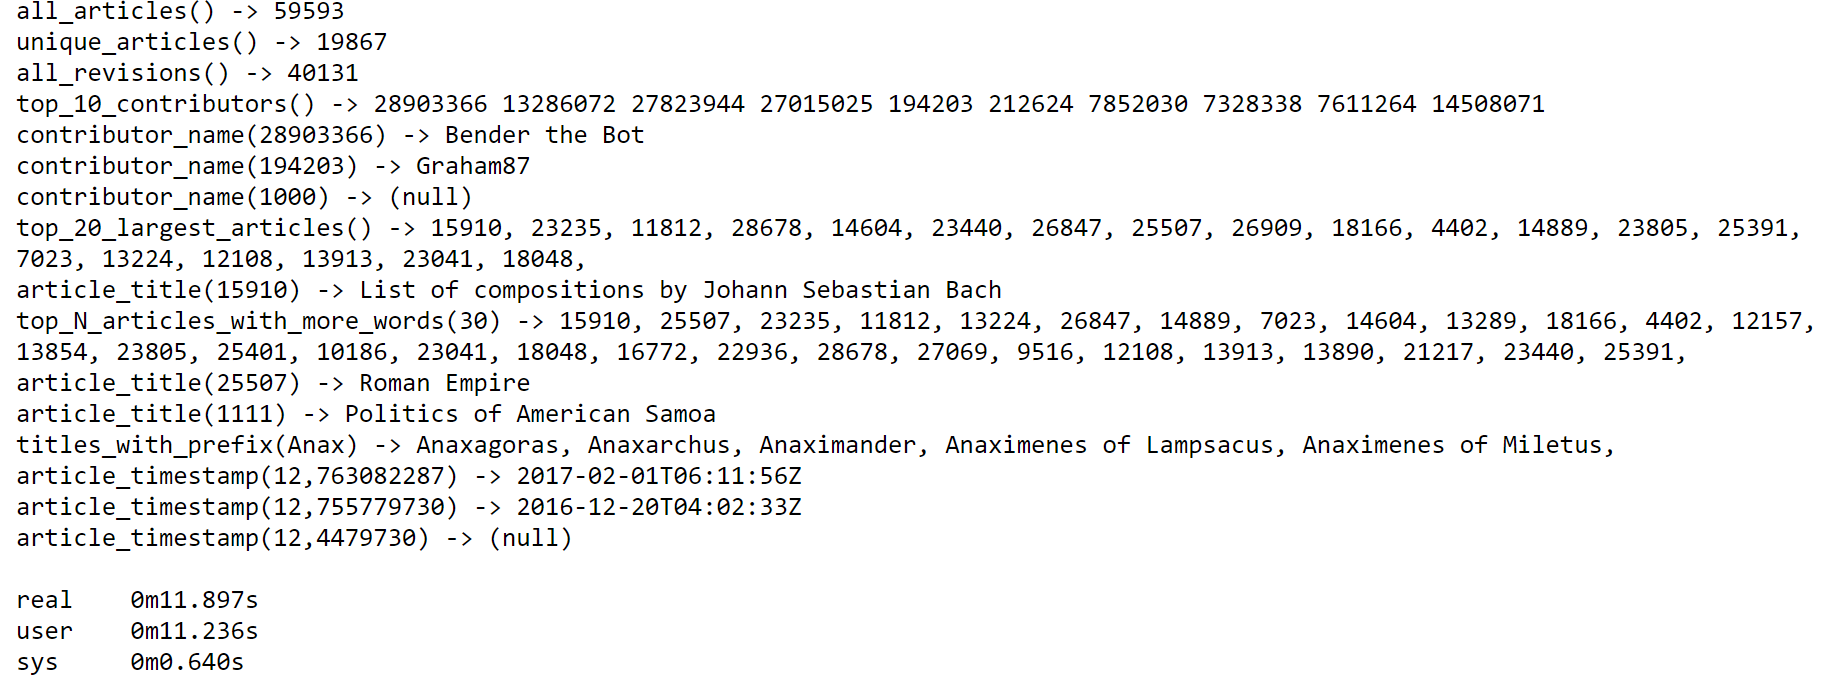
\includegraphics[width = 420pt, height = 230pt]{output}
\end{figure}

\section{Conclusões}
\label{sec:conclusao}
Este projeto serviu para aprofundarmos o conhecimento da linguagem C, assim como as bibliotecas que lhe estão associadas. Achámos que, com a realização de um trabalho deste tipo permite uma consolidação proveitosa da linguagem, não só em termos teóricos como também em termos práticos e acaba por ser uma forma diferente de cimentar os conteúdos de algumas das UCs que nos surgiram neste curso. Permite também melhorar as habilidades na resolução de problemas. Concluímos também que:

\begin{itemize}
        \item O uso da estrutura de dados adequada (hashtables) foi essencial de forma a obter um programa eficiente, que faça a manipulação necessária dos dados em tempo útil;
 	    \item A separação do trabalho em módulos permite uma fácil divisão do trabalho pela equipa, aliando-se ao uso do Git numa organização eficiente do trabalho do grupo.
\end{itemize}

\end{document}